\begin{frame}
	\frametitle{Transazione $\mathfrak{T}$}
	\framesubtitle{struttura dati}
	
	\begin{table}
	  \centering
	  \begin{tabular}{l}
	  	%sia $\orange{\mathfrak{T}_{-1}}$ \textit{precedente} a $\orange{\mathfrak{T}}$ \\
	    $\bullet\;\orange{\mathfrak{T}^{ID}}=\text{hash}(\mathfrak{\orange{T}})$\\
	    $\bullet\;$ timestamp $\orange{t}$ \\ \\
	    \begin{tabular}{l|l}
			$\bullet\;\forall i$ indirizzo di {\color{blue}input}  $\orange{\mathfrak{I}_i^{in}}$ & 
			$\bullet\;\forall j$ indirizzo di {\color{blue}output} $\orange{\mathfrak{I}_j^{out}}$ \\
			\tabitem \sout{somma trasferita $\bitcoinA_i^{in}$} & \tabitem somma ricevuta $\orange{\bitcoinA_j^{out}}$ \\
			\tabitem chiave $\orange{K^{PB}_{i,\,in}}$ & \tabitem $\text{hash}(\orange{K^{PB}_{j,\,out}})$ \\
			\tabitem indice $\orange{p}: \mathfrak{I}_i^{in}=[\mathfrak{I}_p^{out}]_{\orange{\mathfrak{T}_{-1}}}$ \\
			\tabitem $\orange{\mathfrak{T}^{ID}_{-1}}=\text{hash}(\orange{\mathfrak{T}_{-1}})$ \\
			\tabitem firma
			$\orange{\mathfrak{T}^{S_i}}=E(\orange{\tilde{\mathfrak{T}}_i},\,\orange{K^{PR}_{i,\,in}})$
		\end{tabular}		
	  \end{tabular}
	\end{table}

\end{frame}

\begin{frame}
	\frametitle{Transazione $\mathfrak{T}$}
	\framesubtitle{collegamento tra transazioni}

	\begin{figure}[H]
		\begin{center}
			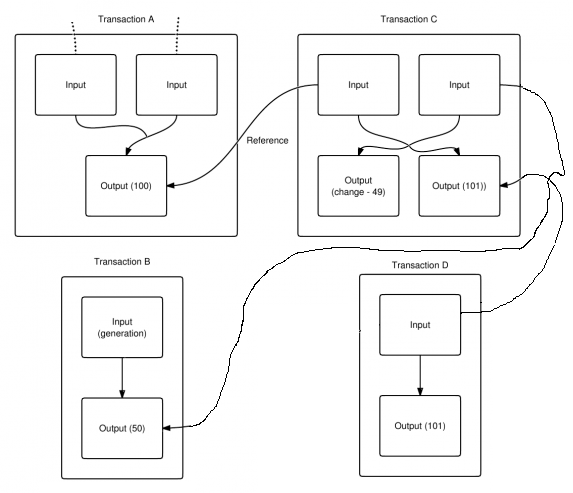
\includegraphics[height = 7 cm]{images/ref.png}	
		\end{center}
	\end{figure}

\end{frame}